%%%%%%%%%%%%%%%%%%%%%%%%%%%%%%%%%%%%%%%%%%%%%%%%%%%%%%%%%%%%%%%%%%%%%%%%%%%%%%%
\section{Design}\label{sec:Design}
%%%%%%%%%%%%%%%%%%%%%%%%%%%%%%%%%%%%%%%%%%%%%%%%%%%%%%%%%%%%%%%%%%%%%%%%%%%%%%%
Here we describe in detail the design and implementation of the KBID system.  First we discuss the high level design where we explain the four major components of the system.  Next, we discuss the interface designs and the communication protocols between the major components.  Finally, we discuss the system workflow.

\subsection{High Level Design}
The system is composed of four main parts: a bracelet (Figure~\ref{fig:bracelet}), an authentication module (Figure~\ref{fig:authenticationmodule}) an authentication client, and a Kerberos authentication server.  The bracelet is a wearable device that fastened to the user's wrist.  The bracelet makes contact with the user's skin and applies a signal directly to the user's skin.  The authentication module has a sensor with a button under it.  When the user touches the sensor and depresses the button, the authentication module initiates communication with the bracelet.  The authentication module is attached via RS-232 serial to the computer system to which the user wants to authenticate.  A workstation hosts the authentication client.  The client monitors the serial connection for data and when necessary, opens a connection to the Kerberos server for authentication.  Finally, the Kerberos server is a default installation and uses the default implementation of the authentication protocol.

\begin{figure}[t]
\centering
\includegraphics[width=0.7\linewidth]{./Bracelet}
\caption[KBID Prototype Bracelet]{KBID Prototype Bracelet}
\label{fig:bracelet}
\end{figure}

\begin{figure}[t]
\centering
\includegraphics[width=0.7\linewidth]{./AuthenticationModule}
\caption[KBID Prototype Authentication Module]{KBID Prototype Authentication Module}
\label{fig:authenticationmodule}
\end{figure}

\subsection{Interfaces and Communication}
The KBID system includes three interfaces.  The interface between the bracelet and the authentication module takes place over the user's skin.  The interface between the authentication module and the authentication client takes place over RS-232 serial.  Finally, the interface between the authentication client and the Kerberos server uses the network.  Since the communication between a client and a Kerberos server is well documented, we will not discuss it in this paper.

\subsubsection{Bracelet to Authentication Module}
%this is the original of the paragraph below
%The communication protocol between the bracelet and the authentication module is a very lightweight protocol.  The messages that the bracelet sends to the authentication modules are called "statuses."  The messages that the authentication module sends to the bracelet are called "commands."  All messages are a series of bytes that are transmitted across the user's skin. A status message had the following structure: [Status ID] [Device ID] [Token Size (in bytes)] [Token].  These fields are delimited by length according to the following table:

The communication protocol between the bracelet and the authentication module is a very lightweight protocol.  The messages that the bracelet sends to the authentication modules are called \emph{statuses}.  The messages that the authentication module sends to the bracelet are called \emph{commands}.  Each message sent over this interface is a length delimited series of bytes. A status message had the following structure: [Status ID] [Device ID] [Data Size (in bytes)] [Data]. The bracelet will send one of two statuses, \emph{authenticated} or \emph{un-authenticated}. If the status is authenticated, the authentication data will be transmitted in the data field.

%\begin{tabular}{|l|l|}
%	\hline  Status ID & 1 Byte \\ 
%	\hline  Device ID & 4 Bytes \\ 
%	\hline  Token Size & 2 Bytes \\ 
%	\hline  Token & 0 to 65535 bytes \\ 
%	\hline 
%\end{tabular} 

%The Status ID will be sent as 0x01 if the bracelet is not authenticated and 0x02 it the bracelet is authenticated.  The Bracelet ID will always be transmitted when the bracelet sends a status.  It is a unique identifier for the specific bracelet.  If the bracelet is not authenticated the Token Size field will be set to 0x00 and the token will be of length 0.  If the bracelet is authenticated then the Token Size field will reflect the length of the token that follows.  Naturally, the token data will be of a length defined by the token size field.

%The next 4 paragraphs and table have been merged into the one that follows them.
%A command message has the following structure: [Command ID] [Device ID] [Payload Size (in bytes)] [Payload].  These fields are delimited by length according to the following table:

%\begin{tabular}{|l|l|}
%	\hline Command ID & 1 byte \\
%	\hline Device ID & 4 bytes long \\
%	\hline Payload Size & 2 Bytes \\
%	\hline Payload & 0 to 65535 bytes \\
%	\hline
%\end{tabular}

%The authentication module will send three commands.  The first command is a "Get Status" command.  This is the only command to which the bracelet will respond.  The Command ID is 0x01, the device ID is set to a special value of 0xFFFFFFFF which the bracelet will regard as a broadcast ID, and the payload size is 0x0000.  The payload is of length 0.  When the bracelet receives as "Get Status" message it responds with a status message.  

%The second command is a "Set Token" command.  The Command ID is 0x02.  The Device ID is set to the ID of the bracelet, and the payload size will be set to the length of the token to be stored.  The token will be appended after the message.  When the bracelet receives a "Set Token" command it will store the payload in memory and set its status to "Authenticated."

%Finally, the authentication module can send a "De-authenticate" command.  The Command ID is set to 0x03 and the Device ID is set to the device of the bracelet to be authenticated.  The Payload Size is 0x00 and the payload is of length 0.  When the bracelet receives this message it will clear any token it has, byte by byte and set its status to "Un-Authenticated."

A command message has the following structure: [Command ID] [Device ID] [Payload Size (in bytes)] [Payload]. The authentication module will send three commands: \emph{Get Status}, \emph{Set Token}, and \emph{De-authenticate}.  A Get Status command causes the bracelet to respond with a status message. A Set Token command causes the bracelet to store the payload in memory as authentication data and set its status to authenticated.  A De-authenticate command causes the bracelet to clear any token it has and set its status to un-authenticated.

\subsubsection{Authentication Module to Authentication Client}

The authentication module and the authentication client communicate status and command messages as well.  The authentication module can send three statuses to the authentication client.  First is the \emph{Un-authenticated Bracelet} message.  This message is sent to the authentication client when the authentication module receives an un-authenticated status from a bracelet.

Next the authentication module can send an \emph{Authenticated Bracelet} status to the authentication client.  It will send this status when the bracelet sends a status of authenticated.  The Authenticated Bracelet status will contain the ticket information that was in the token section of the bracelet's message.

Finally, the authentication module can send a \emph{Ticket Written} status to the authentication client.  This is a message that lets the client know that the ticket information has been successfully written to the bracelet.  

The authentication client sends two commands to the authentication module.  First the \emph{Write Ticket} command.  This instructs the authentication module to pass the ticket included in the command to the bracelet with a Set Token command.  The authentication client can also send a \emph{De-authenticate Bracelet} command.  This instructs the authentication module to issue a De-Authenticate command to the bracelet.

\subsection{System Workflow}
%this is the original of the paragraph below
%The system workflow can be described simply in two use cases.  For the sake of brevity this description of these use cases does not include any error handling.   The first use case is described in Figure 1.  In this use case the user is wearing a bracelet but the bracelet does not yet contain any authentication information.  The users touches the sensor on the authentication module, the authentication module sees that the user's bracelet is not authenticated.  The authentication module tells the authentication client that the user is not authenticated and the client then prompts the user for their username and password.  The client verifies this information with the Kerberos server.  Then instructs the user to touch the sensor on the authentication module again.  The client then instructs the authentication module to write the ticket to the bracelet.  Once the ticket has been written, the client unlocks the workstation.  The message exchange for this use case can be seen in Figure 2.

The system workflow can be described in two use cases.  For the sake of brevity we do not include any error handling.  In the first use case (Figure~\ref{fig:UnauthenticatedME}) the user is wearing a bracelet but the bracelet is not yet authenticated.  The users touches the sensor on the authentication module, the authentication module sees that the user's bracelet is not authenticated and relays this information to the authentication client.  The client prompts the user for their username and password.  The client verifies this information with the Kerberos server, then instructs the user to touch the sensor on the authentication module again.  The client then instructs the authentication module to write the ticket to the bracelet.  Once the ticket has been written, the client unlocks the workstation. 

%\begin{figure}
%\centering
%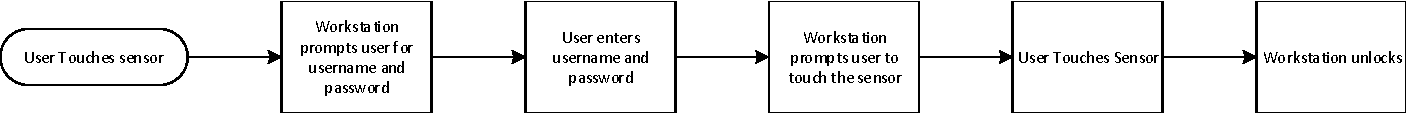
\includegraphics[width=0.7\linewidth]{./UnauthenticatedUC}
%\caption[Un-Authenticated Use Case]{Un-Authenticated Use Case}
%\label{fig:UnauthenticatedUC}
%\end{figure}

\begin{figure}[t]
\centering
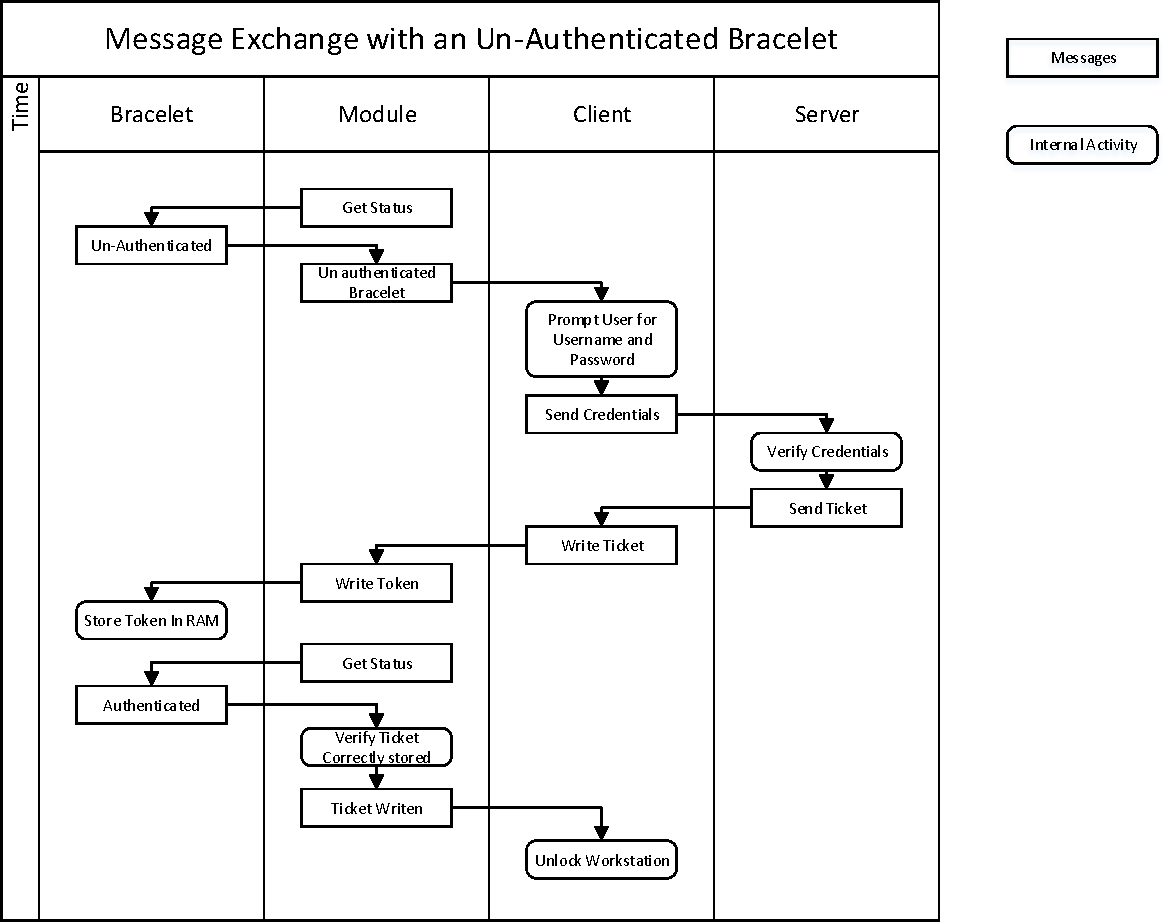
\includegraphics[width=0.7\linewidth]{./UnauthenticatedME}
\caption[Un-Authenticated Message Exchange]{Un-Authenticated Message Exchange}
\label{fig:UnauthenticatedME}
\end{figure}

%this is the original of the paragraph below
%The second use case outlines what happens when the user has a proper token stored in their bracelet.  It is described in Figure 3.  It seems very simple from the user's point of view.  The user touches the sensor on the authentication module and the workstations unlocks.  The process behind the scenes is also much simpler.  The module asks for a status, and the bracelet provides it with the token it has stored.  The module passes this information along to the clients which interoperates the token as a Kerberos ticket.  The client verifies the ticket with the Kerberos server and unlocks the workstation.  The message exchange for this use case is presented in Figure 4.

In the second use case (Figure~\ref{fig:AuthenticatedME}) the user has an authenticated bracelet.  The user touches the sensor on the authentication module.  The module asks for a status, and the bracelet provides it with the token it has stored.  The module passes this information along to the client which interprets the token as a Kerberos ticket.  The client verifies the ticket with the Kerberos server and unlocks the workstation.  Our goal is to perform this use case in less than one second.

%\begin{figure}
%\centering
%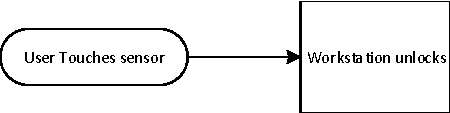
\includegraphics[width=0.25\linewidth]{./AuthenticatedUC}
%\caption[Authenticated Use Case]{Authenticated Use Case}
%\label{fig:AuthenticatedUC}
%\end{figure}

\begin{figure}[t]
\centering
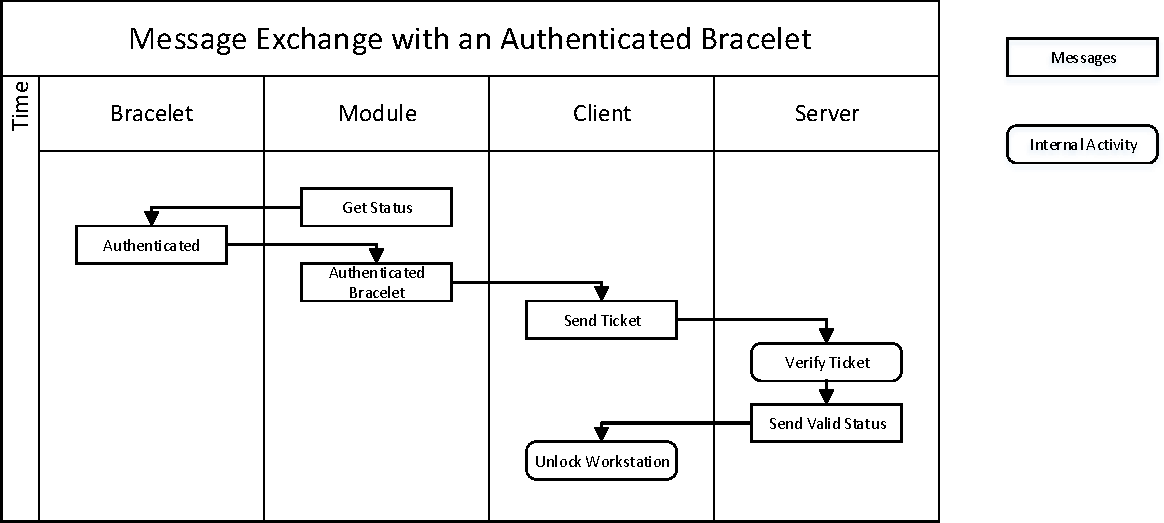
\includegraphics[width=0.7\linewidth]{./AuthenticatedME}
\caption[Authenticated Message Exchange]{Authenticated Message Exchange}
\label{fig:AuthenticatedME}
\end{figure}
